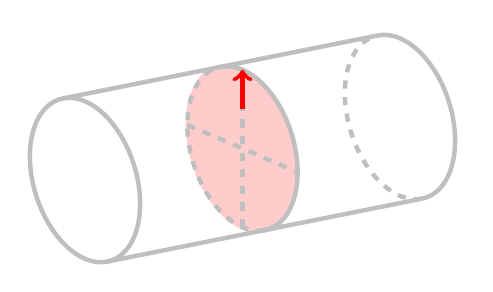
\begin{tikzpicture}
    \begin{scope}[x={(.7cm,-.3cm)},z={(-.5cm,-.1cm)}]
        \path (1,0,0);
        \pgfgetlastxy{\cylxx}{\cylxy}
        \path (0,1,0);
        \pgfgetlastxy{\cylyx}{\cylyy}
        \path (0,0,1);
        \pgfgetlastxy{\cylzx}{\cylzy}
        \pgfmathsetmacro{\cylt}{(\cylzy * \cylyx - \cylzx * \cylyy)/ (\cylzy * \cylxx - \cylzx * \cylxy)}
        \pgfmathsetmacro{\ang}{atan(\cylt)}
        \pgfmathsetmacro{\ct}{1/sqrt(1 + (\cylt)^2)}
        \pgfmathsetmacro{\st}{\cylt * \ct}
        \fill[red!20] (0,0,-4) circle[radius=1.03];
        \begin{scope}[every path/.style={ultra thick,black!25}]

            % front ellipse
            \draw (0,0,0) circle[radius=1];

            % middle ellipse
            \draw (\ct,\st,-4) arc[start angle=\ang,delta angle=180,radius=1];
            \draw[dashed] (\ct,\st,-4) arc[start angle=\ang,delta angle=-180,radius=1];

            % measurement marker in middle of central axis
            \draw[dashed] (-1,0,-4) -- (1,0,-4);
            \draw[dashed] (0,-1,-4) -- (0,1,-4);

            % measurement line
            \draw[->][red] (0,0.5,-4) -- (0,1,-4);

            % Cylinder Edges
            \draw (\ct,\st,0) -- ++(0,0,-8);
            \draw (-\ct,-\st,0) -- ++(0,0,-8);

            % back ellipse
            \draw (\ct,\st,-8) arc[start angle=\ang,delta angle=180,radius=1];
            \draw[dashed] (\ct,\st,-8) arc[start angle=\ang,delta angle=-180,radius=1];
        \end{scope}
    \end{scope}
\end{tikzpicture}
%source: http://tex.stackexchange.com/questions/31548/drawing-simple-3d-cylinders-in-tikz
